\begin{homeworkProblem}

\textbf{Power-Law Distribution:} Implement a Metropolis-Hastings algorithm to simulate from the power-law distributions shown in the lecture.

\solution

The power-law distribution with constant $S=-\dfrac{3}{2}$ is defined as follows:
$$\pi_i=\dfrac{i^S}{\sum\limits_{k=1}^{\infty}k^S}=\dfrac{i^{-\frac{3}{2}}}{\sum\limits_{k=1}^{\infty}k^{-\frac{3}{2}}}\propto i^{-\frac{3}{2}}, \quad\text{for } i=1,2,\ldots$$

Since the state space is $\{1,2,\ldots \}$, which are the positive integers, so the proposal Markov Chain could be constructed with a single reflecting bound:
\begin{center}
\begin{tikzpicture}[->, >=stealth, auto, thick, node distance=2cm]
    \tikzstyle{every state} = [
        fill=blue!20,
        draw=black,
        circle,
        minimum size=30pt,
        font=\large\bfseries
    ]

    \node[state] (1) at (-6, 0) {1};
    \node[state] (2) at (-4,  0) {2};
    \node[state] (3) at (-2,  0) {3};
    \node[state] (4) at (0,  0) {4};
    \node[state, draw=none, fill=none] (ellipsis) at (2,0) {$\cdots$};

    \path (1) edge[bend left=30] node{$1$} (2);
    \path (2) edge[bend left=30] node{$\frac{1}{2}$} (1);
    \path (2) edge[bend left=30] node{$\frac{1}{2}$} (3);
    \path (3) edge[bend left=30] node{$\frac{1}{2}$} (2);
    \path (3) edge[bend left=30] node{$\frac{1}{2}$} (4);
    \path (4) edge[bend left=30] node{$\frac{1}{2}$} (3);
    \path (4) edge[bend left=30] node{$\frac{1}{2}$} (ellipsis);
    \path (ellipsis) edge[bend left=30] node{$\frac{1}{2}$} (4);
\end{tikzpicture}
\end{center}

This is obviously an irreducible Markov Chain, and the transition probability is
$$p_{i,j}=\begin{cases}
\frac{1}{2} & \text{if } j=i\pm 1 \\
1 & \text{if } i=1,j=2 \\
0 & \text{otherwise}
\end{cases}$$
Thus we can apply the Metropolis-Hastings algorithm. \\
For each step, the transition from $i$ to $j$ has the accept rate:
$$a_{i,j} = \min\left(\dfrac{\pi_jp_{j,i}}{\pi_ip_{i,j}},1\right) = \min\left(\dfrac{j^{-\frac{3}{2}}p_{j,i}}{i^{-\frac{3}{2}}p_{i,j}},1\right) \Rightarrow \begin{cases}
a_{1,2} = 2^{-\frac{5}{2}} \\
% a_{2,1} = 1 \\
a_{i,i+1} = \left(\dfrac{i}{i+1}\right)^{\frac{3}{2}} \\
a_{i+1,i} = 1
\end{cases}$$

The number of transition is set to be $1000000$ steps, and the first $10000$ are used as burn in to ensure the state distribution enters the stationary distribution. And the curve for the true distribution and the sampled distribution is shown as follows: \\
\begin{figure}[htbp]
    \centering
    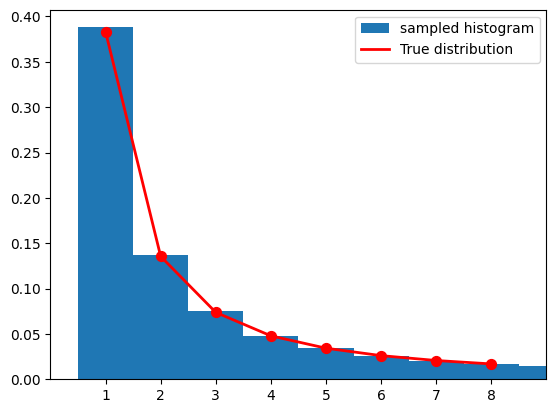
\includegraphics[width=0.45\textwidth]{./figure/p2/distribution.png}
\end{figure}

As for convinence to show, we rounded the numbers into 3 decimal places. The normalize factor used first 1000000 terms to add up. And the numbers of the exact probability and simulated results are shown as follows:
\begin{table}[h]
    \centering
    \begin{tabular}{c ccccccccc}
    \toprule
    i & 1 & 2 & 3 & 4 & 5 & 6 & 7 & 8 & $\geq 9$ \\
    \midrule
    \textbf{Exact}      & 0.383 & 0.135 & 0.074 & 0.048 & 0.034 & 0.026 & 0.021 & 0.017 & 0.262 \\
    \textbf{Simulation} & 0.388 & 0.137 & 0.075 & 0.048 & 0.034 & 0.026 & 0.021 & 0.017 & 0.254 \\
    \bottomrule
    \end{tabular}
\end{table}

And we can see that the simulated results are quite close to the exact results.

\end{homeworkProblem}

\newpage